%! Author = tstreule

\section{Amperometric Sensors}
%%%%%%%%%%%%%%%%%%%%%%%%%%%%%%%%%%%%%%%%%%%%%%%%%%%%%%
%%%%%%%%%%%%%%%%%%%%%%%%%%%%%%%%%%%%%%%%%%%%%%%%%%%%%%
\subsection{Electrochemistry}
%
\formbox{Overpotential}{\eta \equiv \Delta\phi\ped{appl} {-} \Delta\phi^0 \equiv \phi_s {-} \phi_m \equiv E {-} E^0}
{\hfill\scriptsize $E^0$: Nernst}%
\formula{~}{\eta = 0}
\quad (\textbf{equilibrium} i.e. no net current)

\formula{\textbf{Faraday's law}}{
    \textcolor{gray}{
        \textit{1st: } n\propto Q \textit{,\quad 2nd: } \textrm{(equiv. weigth) } W\ped{eq} = M/z
    }
}
\formbox{\textbf{of electrolysis}}{m = \frac{Q}{z\;F}\;M = \frac{I\;t}{z\;F}\;M = n\cdot M}
\enskip \textcolor{gray}{\scriptsize $[m] {=} \unit{g}$, $[n] {=} \unit{mol}$}
%%%%%%%%%%%%%%%%%%%%%%%%%%%%%%%%%%%%%%%%%%%%%%%%%%%%%%
\subsubsection{Butler-Volmer equation \textnormal{Effect of $\eta$ on barrier heigth $G$}}
\label{sec:butler-volmer}
%
\begin{tabular}{r@{:\quad}l}
    Let
    $\phi_s$	& potential of ions in solution\\
    $\phi_m$	& potential of $e^-$ in (metallic) electrode\\
    $z$			& valency of oxidized species\\
    $n$			& \#of transferred $e^-$\\
    $z-n$		& valency of reduced species
\end{tabular}
\formula{\textbf{transfer coeff. $\alpha$}}{nF\eta = n(1-\alpha)F\eta+n\alpha F\eta}
%		\formula{@equilibrium ($\eta=0$)}{k_0 \equiv k\ped{red}=k\ped{ox}}
\scalebox{.9}{%
    \formbox{\fbox{$f{\equiv}\frac{F}{RT} {\overset{@\unit[298]{K}}{=}} \frac{1}{\SI{25.69}{\milli\volt}}$}}{%
        k\ped{red} {=} k_0\;\eu^{-n\alpha f\eta}, \enskip
        k\ped{ox}  {=} k_0\;\eu^{n(1-\alpha)f\eta}
    }	\shortstack[l]{
        @equi. ($\eta=0$)\\
        $k_0 {\equiv} k\ped{red} {=} k\ped{ox}$
    }
}

The Butler-Vomer eq. relates what we measure (the \textbf{current}) with what we would like to determine (the \textbf{concentration} of an analyte):
\scalebox{.9}{%
    \formbox{\textbf{Butler-Volmer}}{j = \underbrace{nFAk_0\vspace{-1mm}}_{\vspace{-2mm}j_0} \big( C\ped{ox}(0,t)\;\eu^{-\alpha nf\eta} - C\ped{red}(0,t)\;\eu^{(1-\alpha)nf\eta} \big)}}
%%%%%%%%%%%%%%%%%%%%%%%%%%%%%%%%%%%%%%%%%%%%%%%%%%%%%%
\subsection{Cyclic Voltammetry}
%
\begin{minipage}{.4\columnwidth}
    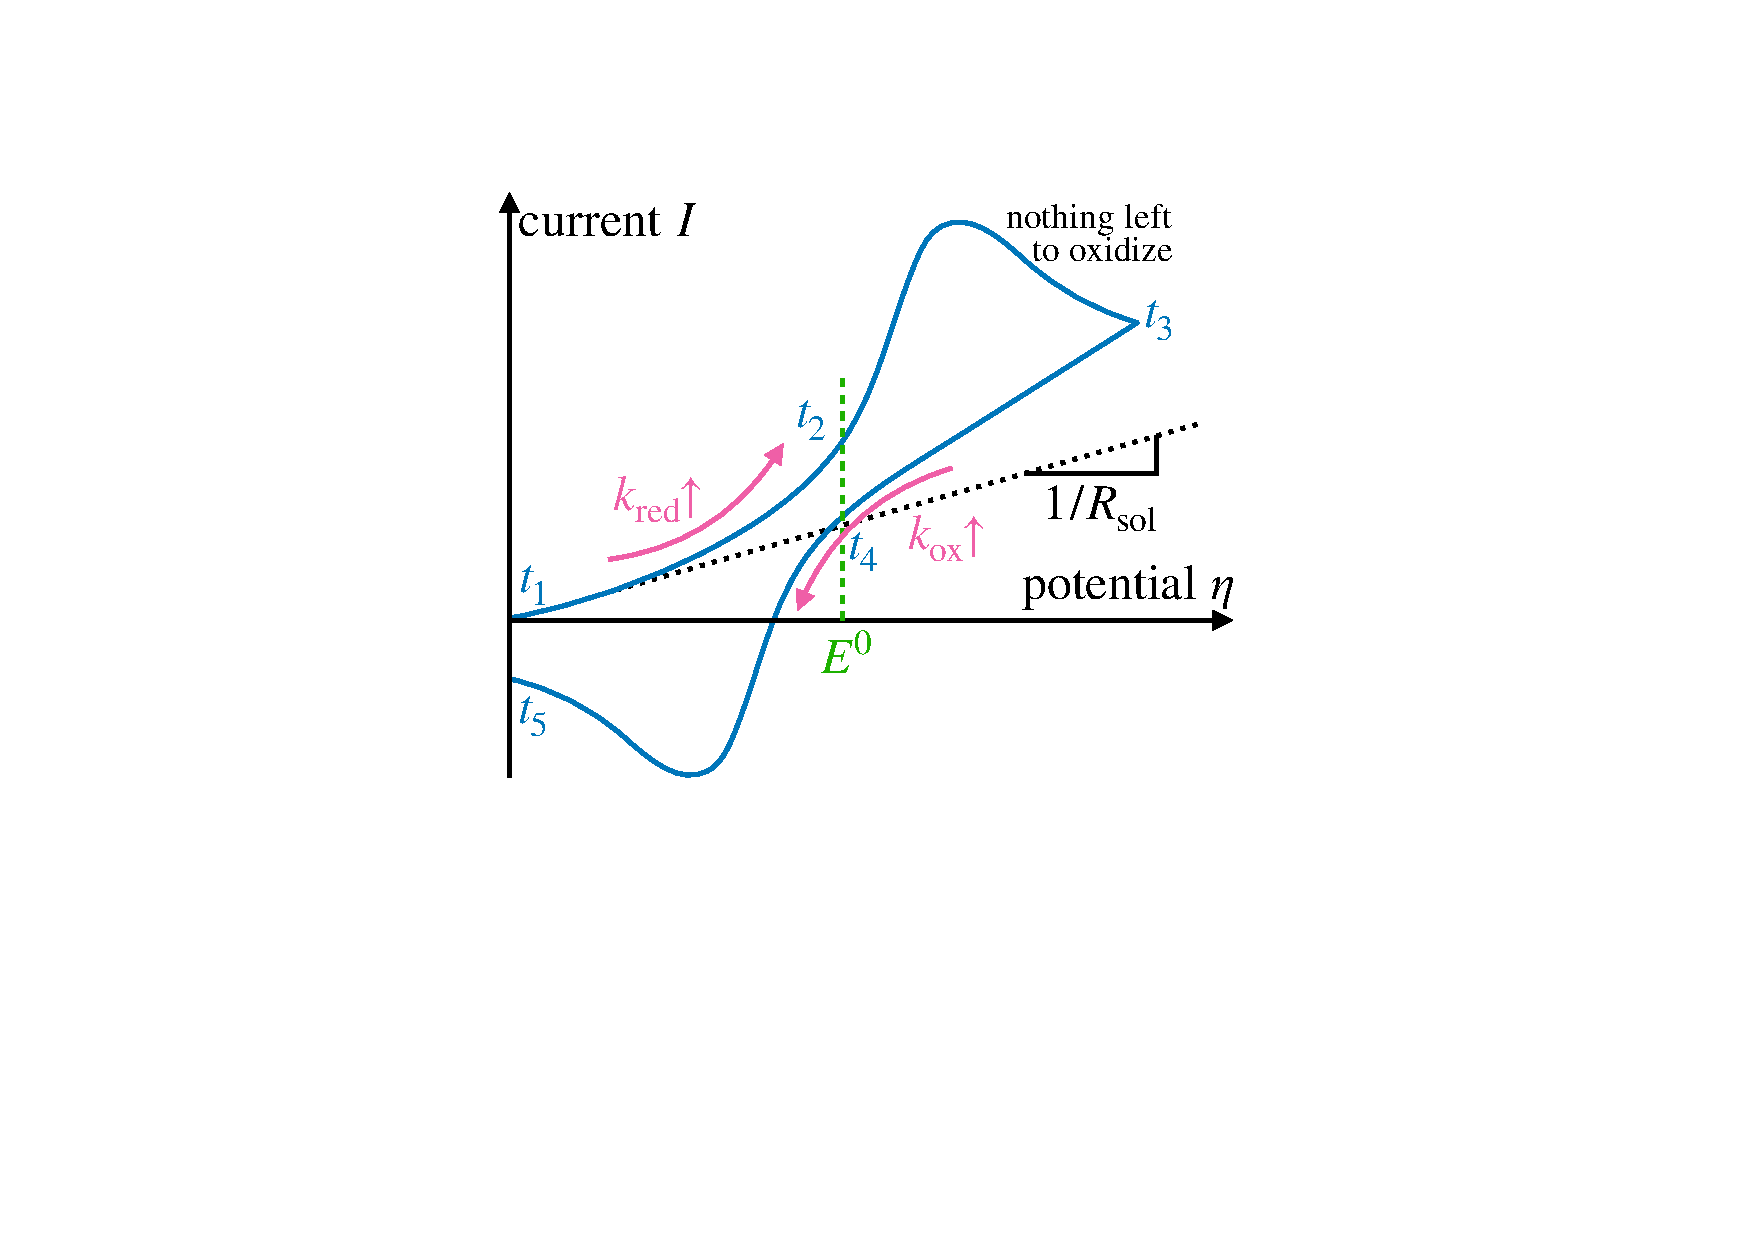
\includegraphics[width=.9\columnwidth]{Electrochemistry_Cyclic_Voltammetry}
\end{minipage}%
\begin{minipage}{.6\columnwidth}
    Offers information on the mechanism of the ec reactions occuring at an electrode.
    \begin{itemize}
        \item May be irreversible\\
        $\to$ \#upper peaks $\neq$ \#lower peaks\\
        $\to$ irreversible reaction fast
        \item Sweep rate\\
        $\to$ irreversible reaction slow
    \end{itemize}
\end{minipage}
\formtex{\textbf{Water electrolysis}}{High potentials/volt's}
%$\to$ affects $I$ %(disturbance, bad)
\formtex{~}{$\to$ affects $I$ (disturbance, bad)}
%%%%%%%%%%%%%%%%%%%%%%%%%%%%%%%%%%%%%%%%%%%%%%%%%%%%%%
\subsection{Amperometric Sensors}
%%%%%%%%%%%%%%%%%%%%%%%%%%%%%%%%%%%%%%%%%%%%%%%%%%%%%%
\subsubsection{Clark \textnormal{(Oxygen)} Electrode \hfill\textnormal{$\to$ Measure \ce{O2}}}
%
\begin{itemize}
    \item test solution \ce{->[O2 passes][membrane]} \ce{Pt} cathode \ce{->[reduction]} current
    \item \ce{Ag} anode is in \ce{KCl} solution ($\to$ ``enough'' \ce{Cl-} for oxidation)
\end{itemize}
%%%%%%%%%%%%%%%%%%%%%%%%%%%%%%%%%%%%%%%%%%%%%%%%%%%%%%
\subsubsection{1st and 2nd Generation}
%
$	\textrm{analyte of interest}
\;\ldots\;
\underbrace{\textrm{redox enzyme}\vspace{-1.5mm}}_{\vspace{-2.5mm}\textrm{catalize}}
\;\underbrace{\ldots\vspace{-.5mm}}_{\vspace{-2.5mm}\textrm{P1}}\;
\underbrace{\textrm{mediator}\vspace{-1mm}}_{\vspace{-2.5mm}\textrm{P2}}
\;\ldots\;
\textrm{Clark Electrode}
$
\formtex{problem P1 (1st)}{\ce{O2} may be consumed, when not measured}
\formtex{problem P2 (2nd)}{need to have ``enough'' of them}
\formtex{Mediator has to be}{$\bullet$ reversible \quad $\bullet$ not toxic \quad $\bullet$ no side reactions}
%%%%%%%%%%%%%%%%%%%%%%%%%%%%%%%%%%%%%%%%%%%%%%%%%%%%%%
\subsubsection{3rd Generation}
%
\textit{Immobilization}/fixation of a redox enzyme on electrode surface

$\to$ free-diffusing redox mediators are not necessary\\
$\to$ in vivo measurments allowed since immobilized

\formtex{problem P3}{Efficient electron transfer (Marcus theory)}\vspace{-1mm}
\formtex{~}{$\to$ may be overcome by mediators}\vspace{-1mm}
\formtex{~}{$\to$ minimize ET distance}
%%%%%%%%%%%%%%%%%%%%%%%%%%%%%%%%%%%%%%%%%%%%%%%%%%%%%%
\subsection{Three Electrode Cell}
%
\begin{minipage}{.5\columnwidth}
    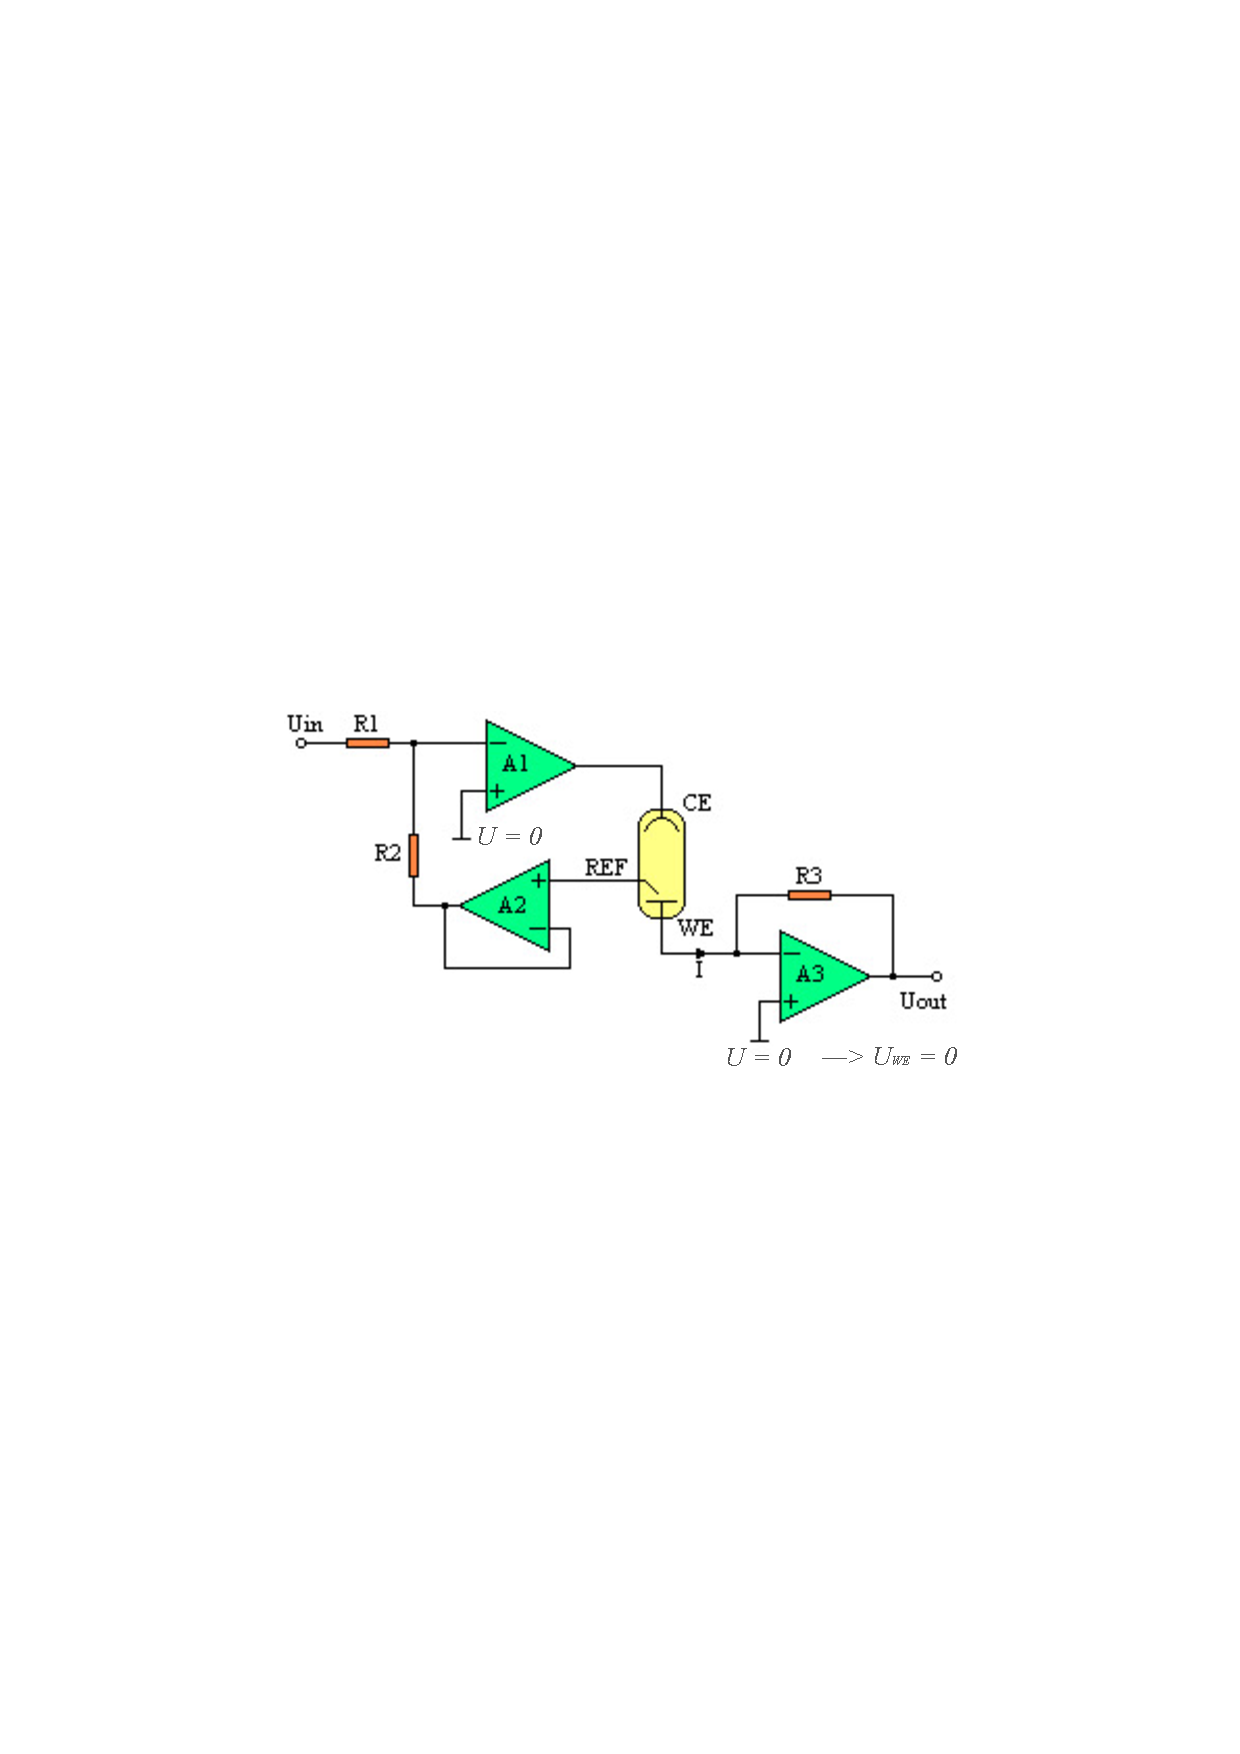
\includegraphics[width=\columnwidth]{Electrochemistry_Three_Electrode_Cell}
\end{minipage}%
\hspace{1cm}
\begin{minipage}{.5\columnwidth-1cm}
    $\frac{U\ped{REF}}{R_2} = - \frac{U\ped{in}}{R_1}$
    \par
    $I = \frac{U\ped{out}}{R_3}$
\end{minipage}
